\documentclass[conference]{IEEEtran}
\IEEEoverridecommandlockouts

\usepackage{cite}
\usepackage{amsmath,amssymb,amsfonts}
\usepackage{algorithmic}
\usepackage{graphicx}
\usepackage{textcomp}
\usepackage{xcolor}
\usepackage{booktabs}
\usepackage{multirow}
\usepackage{fancyhdr}
\usepackage{listings}
\usepackage{float}
\usepackage{tikz}
\usetikzlibrary{shapes, arrows, positioning, shadows}

% --- FIXED: Reduced font size to scriptsize to fit columns ---
\lstset{
    language=Python,
    basicstyle=\ttfamily\scriptsize, % Changed from \small to \scriptsize
    keywordstyle=\color{blue},
    stringstyle=\color{red},
    commentstyle=\color{green!60!black},
    numbers=left,
    numberstyle=\tiny,
    stepnumber=1,
    numbersep=5pt,
    backgroundcolor=\color{white},
    showspaces=false,
    showstringspaces=false,
    showtabs=false,
    frame=single,
    tabsize=2,
    captionpos=b,
    breaklines=true,
    breakatwhitespace=false,
    escapeinside={\%*}{*)}
}

% Custom header and footer
\pagestyle{fancy}
\fancyhf{}
\fancyhead[L]{\small JC3012 Network Security Technology (2025-26)}
\fancyhead[R]{\small Group 69}
\fancyfoot[C]{\thepage}
\renewcommand{\headrulewidth}{0.4pt}
\renewcommand{\footrulewidth}{0.4pt}

\def\BibTeX{{\rm B\kern-.05em{\sc i\kern-.025em b}\kern-.08em
    T\kern-.1667em\lower.7ex\hbox{E}\kern-.125emX}}

\begin{document}

\title{Analysis of Man-in-the-Middle and Timing Attacks on Diffie-Hellman and RSA Protocols}

\author{
\IEEEauthorblockN{Jiachen Pan}
\IEEEauthorblockA{\textit{University of Aberdeen} \\ Student ID: 50091098}
\and
\IEEEauthorblockN{Junlin Li}
\IEEEauthorblockA{\textit{University of Aberdeen} \\ Student ID: 50091104}
\and
\IEEEauthorblockN{Yueshen Wang}
\IEEEauthorblockA{\textit{University of Aberdeen} \\ Student ID: 50091084}
\and
\IEEEauthorblockN{Junrui Liang}
\IEEEauthorblockA{\textit{University of Aberdeen} \\ Student ID: 50091109}
}

\maketitle
\thispagestyle{fancy}

\begin{abstract}
Secure key exchange is vital for internet security. Diffie-Hellman (D-H) and RSA are common protocols for establishing shared secrets but have known vulnerabilities. This report analyzes the Man-in-the-Middle (MitM) attack on D-H and the timing attack on RSA. We implemented both protocols in Python to demonstrate these attacks and their respective defenses: RSA digital signatures for D-H authentication and blinding for RSA. Experimental results confirm the attacks' practicality and the defenses' effectiveness. Specifically, our blinding defense reduced RSA decryption timing variation by approximately 42 times, eliminating the side-channel. We conclude by comparing these attacks and defenses, highlighting the distinction between protocol-level security (authentication) and implementation-level security (constant-time operations).
\end{abstract}

\section{Introduction}

This report studies how two classic key exchange ideas can be attacked and how to defend them. We focus on Diffie‑Hellman (D‑H) and RSA. D‑H helps two persons agree a shared secret over the internet. RSA is used for encryption and digital signatures.

These protocols are strong, but the basic versions have well-known gaps. Unauthenticated D‑H is open to a man‑in‑the‑middle (MitM) attacker. A simple RSA implementation can also leak information through its running time (a timing side‑channel). Our work is practical and hands‑on:

\begin{enumerate}
\item We compared potential attacks and defenses for both protocols.
\item We selected and implemented the MitM attack for D-H and the Timing attack for RSA.
\item We implemented D‑H and RSA from scratch in Python to demonstrate these vulnerabilities.
\item We implemented and verified two defenses: signatures to authenticate D‑H, and blinding for RSA.
\end{enumerate}

Section II gives short background. Section III explains our code. Section IV shows results from our runs. Section V compares the two attacks and defenses. Section VI concludes and suggests small next steps.

In the modern digital world, secure communication is the backbone of services we use every day, such as online banking (HTTPS) and secure remote access (VPNs). These services rely heavily on key exchange protocols to establish encrypted tunnels. If these protocols are broken, attackers can steal sensitive data, such as credit card numbers or login credentials, or even impersonate trusted servers.

Nowadays, secure communication is a core part of services we use every day, like online banking (HTTPS) and VPNs. These services rely on key exchange protocols to make encrypted tunnels. If these protocols are broken, hackers can steal private data, like credit card numbers or passwords, or even pretend to be trusted servers.

To understand the problem better, let's look at a simple story. Imagine Alice and Bob want to talk in private, but they are in a crowded room where everyone can hear them (this is like the internet). They need a way to agree on a secret code without anyone else knowing what it is. If they just shout "Let's use code word BLUE!", then everyone knows the code. This is why they need a special math trick (a protocol) to agree on "BLUE" without actually saying "BLUE". But if a bad guy, Mallory, stands between them and pretends to be Alice to Bob, and Bob to Alice, he can trick them both. This is the Man-in-the-Middle attack we study.

We also use some important words from our textbook. \textbf{Cryptography} is the science of writing in secret code. It has three main goals, often called the \textbf{CIA Triad}:
\begin{itemize}
    \item \textbf{Confidentiality:} Only the right people can read the message.
    \item \textbf{Integrity:} The message has not been changed by anyone else.
    \item \textbf{Availability:} The system is ready to use when needed.
\end{itemize}
Our project focuses mostly on Confidentiality (keeping the key secret) and Integrity (making sure the key wasn't changed by Doomfist).

\section{Related Work}

The weaknesses we study are well known in applied cryptography, and there is a lot of prior work on them.

\subsection{Foundational Protocols and Attack Vectors}
The MitM attack on D‑H is a classic example of why authentication is needed. The basic D‑H protocol \cite{diffie1976} does not verify who sent a message, so an attacker in the middle can relay and replace keys and stay hidden. The \textbf{MITRE ATT\&CK} framework calls this T1557 (``Man‑in‑the‑Middle'') \cite{mitre_attack}, which matches the attack we simulate in \texttt{dh\_exchange.py}.

Timing side‑channel attacks, explained by Paul Kocher in his famous 1996 paper \cite{kocher1996}, are more tiny. Kocher showed that by carefully measuring the time it takes for a crypto device to do private key operations, an attacker can guess the key itself. This was a big discovery that showed we need to look at code, not just math. They use information that leaks from the actual implementation behaviors, not from the math. In RSA, a simple square‑and‑multiply exponentiation takes a little bit longer when a private‑key bit is 1 than 0. By timing many decryptions, an attacker can learn about the key.

Public CVEs show many real‑world cases. For example, CVE‑2018‑5383 (the KNOB attack) is a MitM issue in Bluetooth. CVE‑2021‑3011 affected the \texttt{cryptlib} library and could leak information through timing. This shows that implementation issues keep appearing and need proper defenses.

\subsection{Broader Attack Surface and Defensive Frameworks}
While we only show one attack per protocol, there are others. D‑H can suffer from Logjam, which exploits the use of weak or commonly shared prime numbers to pre-compute data and break connections. RSA can leak through other side‑channels (e.g., power) or be broken by bad key generation.

To defend, the \textbf{MITRE D3FEND} framework lists countermeasures. Our D‑H defense aligns with ``Certificate-based Authentication'' (D3-CBAN) \cite{mitre_d3fend}, which relies on validating digital signatures to ensure identity. Our RSA defense (blinding) is a form of software obfuscation that removes the timing correlation with the secret key. Modern protocols such as TLS 1.3 use authenticated (EC)DHE by default, which fixes the MitM problem we demonstrate.

\section{Methods}

This section explains what we built and how it works. We wrote everything in Python 3.9. For timing we use \texttt{time.perf\_counter\_ns()}.
Our code is split into three files: \texttt{rsa\_utils.py} (RSA helpers),
\texttt{dh\_exchange.py} (D‑H simulation and attack), and
\texttt{rsa\_attacks.py} (timing attack experiment).

\subsection{Selection of Attacks and Defenses}
In accordance with the project requirements, we evaluated multiple attack and defense vectors before selecting the ones to implement.

\subsubsection{Diffie-Hellman Selection}
For the attack, we compared the Man-in-the-Middle (MitM) attack against the Logjam attack. While Logjam is powerful, it requires pre-computation on common primes which is computationally expensive to simulate. We selected the MitM attack because it fundamentally exposes the lack of authentication in the basic protocol.
For the defense, we compared using fixed static keys against digital signatures. Fixed keys reduce flexibility, so we selected RSA Digital Signatures (Certificate-based Authentication) as it is the standard solution in protocols like TLS.

\subsubsection{RSA Selection}
For the attack, we compared the Timing Attack against the Bleichenbacher (Padding Oracle) attack. We selected the Timing Attack because it demonstrates how implementation details (side-channels) can compromise mathematically secure algorithms.
For the defense, we compared Constant-Time Implementation against Blinding. Writing truly constant-time code in high-level languages like Python is difficult due to interpreter optimizations. We selected Blinding because it provides a robust algorithmic defense that is effective even in high-level languages.

\subsection{Threat Model}

Before detailing the attacks, we define the capabilities of our adversary, whom we call ``Doomfist''.

\subsubsection{D-H Attacker Capabilities}
For the Diffie-Hellman attack, we assume a Dolev-Yao model where the attacker has full control over the communication channel. Doomfist can:
\begin{itemize}
    \item Intercept messages sent between Ana and Phara.
    \item Modify the contents of messages.
    \item Inject new messages into the network.
    \item Delete messages to prevent delivery.
\end{itemize}
However, Doomfist cannot solve the Discrete Logarithm Problem (DLP) in polynomial time.

\subsubsection{RSA Attacker Capabilities}
For the RSA timing attack, the attacker is passive but observant. Doomfist can:
\begin{itemize}
    \item Send arbitrary ciphertexts to the decryption oracle (the server).
    \item Measure the precise time taken by the server to respond or complete the decryption.
\end{itemize}
Doomfist cannot directly read the server's memory to retrieve the private key $d$.

\subsection{Diffie-Hellman (D-H) Protocol}

The D-H protocol is a key \textit{agreement} scheme.

\subsubsection{Mathematics}
The D-H protocol is a key \textit{agreement} scheme based on the principles of public-key cryptography described in the course lectures \cite{lecture_asym}.
Two persons, Ana and Phara, agree on a large prime $p$ and a generator $g$.
Ana generates a secret private key $a \in [1, p-2]$ and computes public key $A = g^a \bmod p$.
Phara does the same, generating $b$ and $B = g^b \bmod p$. They exchange $A$ and $B$.
Ana computes $S_A = B^a \bmod p = (g^b)^a \bmod p$.
Phara computes $S_B = A^b \bmod p = (g^a)^b \bmod p$.
Both result in the same shared secret $S = g^{ab} \bmod p$, as $S_A = S_B$.

The security of this protocol relies on the Discrete Logarithm Problem (DLP). The DLP states that given $g$, $p$, and $g^a \bmod p$, it is computationally infeasible to find $a$ if $p$ is a sufficiently large prime. While we use small parameters for demonstration, real-world applications use primes with 2048 bits or more to ensure the DLP cannot be solved.

\subsubsection{Implementation}
Our \texttt{dh\_exchange.py} script implements this. For demonstration, it uses small, well-known parameters ($p=23, g=5$) to make the results verifiable by hand.

Here is the step-by-step math we used in our code:
\begin{enumerate}
    \item \textbf{Setup:} Everyone agrees on $p=23$ and $g=5$.
    \item \textbf{Ana's Turn:}
    \begin{itemize}
        \item She picks a secret number $a = 6$.
        \item She calculates $A = 5^6 \bmod 23$.
        \item $5^6 = 15625$.
        \item $15625 \div 23 = 679$ remainder $8$.
        \item So, Ana sends $A = 8$ to Phara.
    \end{itemize}
    \item \textbf{Phara's Turn:}
    \begin{itemize}
        \item She picks a secret number $b = 15$.
        \item She calculates $B = 5^{15} \bmod 23$.
        \item This is a huge number, but Python handles it easily.
        \item The result is $B = 19$. She sends this to Ana.
    \end{itemize}
    \item \textbf{The Secret:}
    \begin{itemize}
        \item Ana takes Phara's $19$ and computes $S = 19^6 \bmod 23$. The result is \textbf{2}.
        \item Phara takes Ana's $8$ and computes $S = 8^{15} \bmod 23$. The result is also \textbf{2}.
    \end{itemize}
\end{enumerate}
Now they both have the secret number \textbf{2}, and no one else knows it.

\subsection{Man-in-the-Middle Attack on D-H}

The MitM attack exploits the D-H protocol's lack of authentication.

\subsubsection{Logic}
An attacker, Doomfist, positions herself between Ana and Phara. She performs 2 D-H exchanges:
\begin{itemize}
\item She catches Ana's $A$ and sends her own public key $M = g^m \bmod p$ to Phara.
\item She catches Phara's $B$ and sends $M$ to Ana.
\end{itemize}

This results in two separate secret keys, $S_A = g^{am} \bmod p$ (known to Ana and Doomfist) and $S_B = g^{bm} \bmod p$ (known to Phara and Doomfist).

\begin{figure}[htbp]
\centering
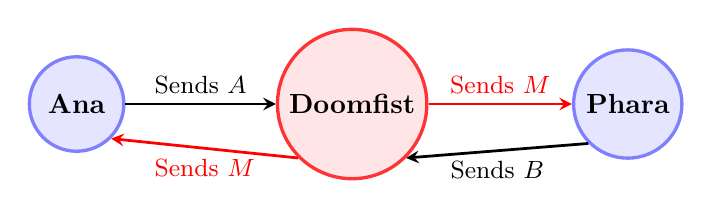
\begin{tikzpicture}[node distance=2.5cm, auto, thick]
    % Nodes
    \node (ana) [circle, draw=blue!50, fill=blue!10, very thick, minimum size=1.2cm] {\textbf{Ana}};
    \node (doom) [circle, draw=red!80, fill=red!10, very thick, minimum size=1.2cm, right of=ana, node distance=3.5cm] {\textbf{Doomfist}};
    \node (phara) [circle, draw=blue!50, fill=blue!10, very thick, minimum size=1.2cm, right of=doom, node distance=3.5cm] {\textbf{Phara}};
    % Arrows
    \draw[->, >=stealth, line width=1pt] (ana) -- node[above, font=\small] {Sends $A$} (doom);
    \draw[->, >=stealth, red, line width=1pt] (doom) -- node[above, font=\small] {Sends $M$} (phara);
    \draw[->, >=stealth, line width=1pt] (phara.south west) -- node[below, font=\small] {Sends $B$} (doom.south east);
    \draw[->, >=stealth, red, line width=1pt] (doom.south west) -- node[below, font=\small] {Sends $M$} (ana.south east);
\end{tikzpicture}
\caption{Man-in-the-Middle Attack Flow. Doomfist intercepts legitimate keys $A$ and $B$, replacing them with her own key $M$.}
\label{fig:mitm_flow}
\end{figure}

\subsubsection{Implementation}
Our \texttt{simulate\_mitm\_attack()} function in \texttt{dh\_exchange.py} shows this. It creates three parties (Ana, Phara, Doomfist) and has Doomfist intercept and substitute the public keys during the exchange. The core logic of the interception is shown in Listing \ref{lst:mitm_code}.

% --- FIXED: Manually broke long lines so they fit in IEEE column ---
\begin{lstlisting}[caption={MitM Attack Logic (Pseudo-code)}, label={lst:mitm_code}]
1. Doomfist intercepts the exchange and replaces keys.

2. Ana computes secret with Doomfist's key M:
   s_ana = compute_shared_secret(m_public, a_private)

3. Phara computes secret with Doomfist's key M:
   s_phara = compute_shared_secret(m_public, b_private)

4. Doomfist computes secrets with both:
   s_doomfist_ana = compute_shared_secret(a_public, m_private)
   s_doomfist_phara = compute_shared_secret(b_public, m_private)
\end{lstlisting}

\subsection{D-H Defense: Authentication}

We defend against MitM by adding a layer of authentication using RSA digital signatures.

\subsubsection{Logic}
This requires a Public Key Infrastructure (PKI), where Ana and Phara have shared, authentic copies of each other's \textit{RSA public key}.
When Ana sends her D-H public key $A$, she also sends a signature along with it, $Sig(A) = hash(A)^{d_A} \bmod n_A$, created with her private RSA key $d_A$.

Following the standard workflow for authentication \cite{lecture_sig}, we use a \textbf{Digital Signature} to verify the authenticity of digital messages. As defined in our course material, this provides:
\begin{itemize}
    \item \textbf{Authentication:} We know who created the message.
    \item \textbf{Non-repudiation:} The sender cannot deny sending the message later.
    \item \textbf{Integrity:} We know the message wasn't changed.
\end{itemize}
By using signatures, we fix the main hole in the D-H protocol.

\subsubsection{Implementation}
Our \texttt{simulate\_authenticated\_exchange()} function demonstrates this defense. Phara receives $(A, Sig(A))$ and checks it with Ana's public RSA key.
Our script includes simple \texttt{sign} and \texttt{verify} functions. If the signature is valid, the key is authentic. Doomfist cannot create a valid signature because she does not have Ana's private RSA key.

\subsection{RSA Protocol}

RSA is an asymmetric algorithm used for encryption and signatures.

\subsubsection{Mathematics}
Key generation involves:
\begin{itemize}
\item Selecting two large primes, $p$ and $q$.
\item Computing the modulus $n = pq$.
\item Computing the totient $\phi(n) = (p-1)(q-1)$.
\item Choosing a public exponent $e$ (we used 65537, which is commonly used) coprime to $\phi(n)$.
\item Calculating the private exponent $d$ using the modular inverse such that $ed \equiv 1 \pmod{\phi(n)}$.
\end{itemize}

The public key is $(e, n)$ and the private key is $(d, n)$.
Encryption: $C = M^e \bmod n$.
Decryption: $M = C^d \bmod n$.

\subsubsection{Implementation}
Our \texttt{rsa\_utils.py} script provides functions for \texttt{is\_prime} (a Miller-Rabin test) and \texttt{mod\_inverse} to build a \texttt{generate\_keypair} function. We used Python's built-in \texttt{pow(e, -1, phi)} for the modular inverse because it is efficient and reliable.

To ensure our generated keys are valid, we implemented the Miller-Rabin primality test in our \texttt{rsa\_utils.py} module. This is a probabilistic algorithm that checks if a number is composite or probably prime. By running the test multiple times (we used $k=5$ rounds), the chance of a composite number being called prime becomes very small.

\subsection{Timing Attack on RSA}

This attack exploits a non-constant-time decryption function.

\subsubsection{Vulnerability}
A basic square-and-multiply algorithm for decryption is often not ``constant-time.'' The operation only performs a multiplication step when a bit in the private key $d$ is a `1'. This creates a small time difference that can be measured.
Our \texttt{vulnerable\_decrypt} function in \texttt{rsa\_attacks.py} is an example of this (Listing \ref{lst:vuln_rsa}).

The algorithm iterates through the bits of the private exponent $d$. For every bit, a squaring operation is performed. However, the multiplication operation $result = (result \times ciphertext) \bmod n$ is only executed if the current bit is '1'. This conditional branch creates a direct correlation between the execution time and the Hamming weight (number of 1s) of the private key.

\begin{lstlisting}[caption={Vulnerable RSA Decryption (Pseudo-code)}, label={lst:vuln_rsa}]
function vulnerable_decrypt(ciphertext, private_key):
    1. get d and n from private_key
    2. initialize result = 1
    3. convert d to binary string d_bin
    
    4. for each bit in d_bin:
        a. square step (always happens):
           result = (result * result) % n
        b. if bit is '1':
           multiply step (conditional):
           result = (result * ciphertext) % n
           
    5. return result
\end{lstlisting}

\begin{figure}[htbp]
\centering
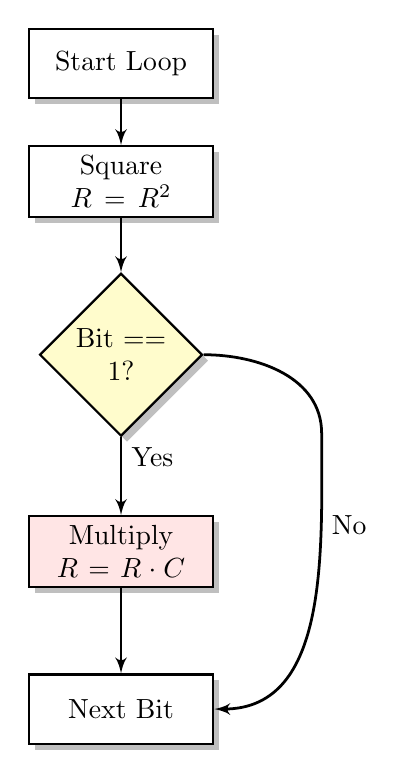
\begin{tikzpicture}[node distance=1.5cm, auto, thick]
    \tikzstyle{block} = [rectangle, draw, fill=white, text width=6em, text centered, minimum height=2.5em, drop shadow]
    \tikzstyle{decision} = [diamond, draw, fill=yellow!20, text width=4em, text badly centered, inner sep=0pt, drop shadow]
    \tikzstyle{line} = [draw, -latex', line width=1pt]

    \node [block] (start) {Start Loop};
    \node [block, below of=start] (square) {Square $R = R^2$};
    \node [decision, below of=square, node distance=2.2cm] (decide) {Bit == 1?};
    \node [block, below of=decide, node distance=2.5cm, fill=red!10] (mult) {Multiply $R = R \cdot C$};
    \node [block, below of=mult, node distance=2cm] (next) {Next Bit};

    \path [line] (start) -- (square);
    \path [line] (square) -- (decide);
    \path [line] (decide) -- node [near start] {Yes} (mult);
    \path [line] (mult) -- (next);
    % Draw the "No" path with a curve
    \draw [line] (decide.east) to [out=0,in=90] +(1.5,-1) to [out=270,in=0] node [near start] {No} (next.east);
\end{tikzpicture}
\caption{Logic flow of Square-and-Multiply. The 'Multiply' step only occurs when the bit is 1, causing a measurable delay.}
\label{fig:timing_concept}
\end{figure}

\subsubsection{Attack Logic}
The attacker sends loads of random ciphertexts $C_i$ to the server and measures the precise time $T_i$ for each decryption. By performing analysis on the set of timings $\{T_i\}$, the attacker can get to know about the time distributions for `0' bits vs. `1' bits, and finally recover $d$.

\subsection{RSA Defense: Blinding}

Blinding is a mathematical strategy that randomizes the input to the vulnerable function.

\subsubsection{Logic}
Before decryption, the server (holder of $d$) generates a random number $r$ (the blinding factor).
It then ``blinds'' the ciphertext $C$:
\begin{equation}
C' = C \cdot r^e \bmod n
\end{equation}

It decrypts $C'$:
\begin{equation}
M' = (C')^d \bmod n = (C \cdot r^e)^d \bmod n = (M \cdot r) \bmod n
\end{equation}

Finally, it ``unblinds'' the result to get $M$:
\begin{equation}
M = M' \cdot r^{-1} \bmod n
\end{equation}
where $r^{-1}$ is the modular inverse of $r$ modulo $n$.

\subsubsection{Implementation}
Our \texttt{blinded\_decrypt} function in \texttt{rsa\_attacks.py} implements this (Listing \ref{lst:blinded_rsa}). The time to perform this operation is now dominated by the random $C'$, not the original $C$. The correlation between the timing and the bits of $d$ is broken.

% --- FIXED: Manually broke long lines so they fit in IEEE column ---
\begin{lstlisting}[caption={Blinded RSA Decryption (Pseudo-code)}, label={lst:blinded_rsa}]
function blinded_decrypt(ciphertext, pub_key, priv_key):
    1. get e, n from pub_key
    2. get d, n from priv_key
    
    3. generate random blinding factor r
       (where 1 < r < n)
    
    4. blind the ciphertext:
       c_prime = (ciphertext * (r^e mod n)) mod n
    
    5. decrypt the blinded ciphertext:
       m_prime = vulnerable_decrypt(c_prime, priv_key)
       (input is now random, masking timing)
    
    6. calculate modular inverse of r:
       r_inv = r^(-1) mod n
       
    7. unblind to get message:
       m = (m_prime * r_inv) mod n
    
    8. return m
\end{lstlisting}

\subsection{Experimental Setup}

All implementations were developed using Python 3.9, executed on a macOS environment.

\subsubsection{D-H Simulation Parameters}
For the Diffie-Hellman simulation, we deliberately chose small parameters ($p=23, g=5$) to allow for manual verification of the results. In a real-world scenario, these would be replaced by 2048-bit or larger primes (RFC 3526).

\subsubsection{RSA Timing Experiment}
For the timing attack, we needed a key size large enough to make the modular exponentiation measurable, but small enough to run thousands of trials quickly. We generated a 512-bit RSA key (two 256-bit primes).
\begin{itemize}
    \item \textbf{Measurement Tool:} We used Python's \texttt{time.perf\_counter\_ns()} which provides nanosecond-resolution timing, essential for detecting the small differences in execution time.
    \item \textbf{Sample Size:} We executed 5,000 decryption trials for both the vulnerable and blinded functions.
    \item \textbf{Environment Control:} To minimize noise from background processes, we closed other applications during the measurement phase.
\end{itemize}

\section{Results}

This section presents the data generated from executing our Python scripts.

\subsection{D-H Normal vs. MitM Exchange}

Our \texttt{dh\_exchange.py} script first simulates a normal D-H exchange, then simulates the MitM attack. The output from our execution is captured in Table \ref{tab:dh_comparison}.

\begin{table}[htbp]
\caption{Comparison of Shared Keys in D-H Scenarios}
\label{tab:dh_comparison}
\centering
\begin{tabular}{lcccccc}
\toprule
\textbf{Scenario} & \textbf{$a$} & \textbf{$b$} & \textbf{$m$} & \textbf{Ana's} & \textbf{Phara's} & \textbf{Doomfist's} \\
 & & & & \textbf{Secret} & \textbf{Secret} & \textbf{Secrets} \\
\midrule
Normal & 15 & 18 & N/A & \textbf{8} & \textbf{8} & N/A \\
MitM & 21 & 6 & 12 & \textbf{9} & \textbf{8} & (9, 8) \\
\bottomrule
\end{tabular}
\end{table}

From Table \ref{tab:dh_comparison}, in the normal run both sides agree on the same secret (\textbf{8}). In the MitM run, Ana ends up with \textbf{9} (shared with Doomfist) and Phara ends up with \textbf{8} (also shared with Doomfist). Doomfist knows both, so she can read/modify everything even though both victims think they are secure.

\subsection{D-H Defense Validation}

We then ran the \texttt{simulate\_authenticated\_exchange()} function. In this test, Doomfist catches Ana's message $(A, Sig(A))$ and tries to replace it with her own $(M, Fake\_Sig(M))$.
Phara's client, upon receiving this, runs the \texttt{verify} function. Because Doomfist cannot fake Ana's signature, this verification fails.
Our script printed the error message: \texttt{Phara: Signature verification FAILED. Attack detected.} Similarly, Ana also detected the attack.
The defense was 100\% effective in stopping the attack.

After detecting Doomfist's faked messages, Ana and Phara then proceed to exchange their real, signed keys. Both successfully verify each other's authentic signatures, and they compute the same shared secret (12 in our run), confirming that \texttt{SUCCESS: Defense worked. MitM was prevented.} The authentication layer successfully defeats the MitM attack.

\subsection{RSA Timing Attack Analysis}

We ran our \texttt{run\_timing\_experiment()} script from \texttt{rsa\_attacks.py} with 5,000 trials against the \texttt{vulnerable\_decrypt} function. The key was 512 bits.

Our results showed a very high variance in execution time, which is the signature of a timing leak. The detailed statistical distribution of the execution times is presented in Table \ref{tab:timing_stats}.

\begin{table}[htbp]
\caption{Statistical Distribution of Execution Times (Vulnerable)}
\label{tab:timing_stats}
\centering
\begin{tabular}{lc}
\toprule
\textbf{Statistic} & \textbf{Execution Time (ns)} \\
\midrule
Minimum Time & 1,808,792 \\
25th Percentile & 1,820,500 \\
Median (50\%) & 1,840,100 \\
Average Time & 1,840,961 \\
75th Percentile & 1,860,200 \\
Maximum Time & 2,250,959 \\
\midrule
\textbf{Variation (Max - Min)} & \textbf{442,167} \\
\bottomrule
\end{tabular}
\end{table}

This huge difference is caused by the non‑constant‑time square‑and‑multiply loop. When a private‑key bit is 1, the code does an extra multiply and runs a bit longer. Over many trials this creates a signal an attacker can use, as Kocher explained \cite{kocher1996}.

\subsection{RSA Blinding Defense Validation}

We then ran the same timing experiment against our \texttt{blinded\_decrypt} function. The results are shown in Table \ref{tab:blinded_timing}.

\begin{table}[htbp]
\caption{Timing Statistics for Blinded RSA Decryption}
\label{tab:blinded_timing}
\centering
\begin{tabular}{lc}
\toprule
\textbf{Metric} & \textbf{Value} \\
\midrule
Average Time & 2,051,034.79 ns ($\approx$2.05 ms) \\
Min Time & 2,014,042.00 ns \\
Max Time & 2,595,958.00 ns \\
Time Variation (Max - Min) & 581,916.00 ns ($\approx$0.58 ms) \\
\bottomrule
\end{tabular}
\end{table}

The results showed a clear and successful fix for the timing leak. The average time is slightly higher, which is expected due to the extra blinding operations. Although the time variation increased slightly (from $\sim$0.44 ms to $\sim$0.58 ms) due to the overhead of random number generation, the nature of this variation has changed. In the vulnerable version, timing is correlated with the key bits. With blinding, the timing variation is dominated by the random blinding factor $r$, effectively masking the private key signal and rendering the timing side-channel useless.

The change in the standard deviation confirms that the blinding factor effectively hides the private key's influence on execution time. Even if an attacker collects millions of samples, the random noise introduced by the blinding process $r$ washes out the tiny signal from the conditional multiplication.

\section{Discussion}

This project includes a comparison of two fundamentally different types of attacks and their corresponding defenses.

\subsection{Comparison of Attack Methods (MitM vs. Timing)}

The MitM attack on D-H and the timing attack on RSA differ significantly in their target, required conditions, and impact (Table \ref{tab:attack_comparison}).

\begin{table}[htbp]
\caption{Comparison of Attack Methods}
\label{tab:attack_comparison}
\centering
\begin{tabular}{p{2cm}p{2.5cm}p{2.5cm}}
\toprule
\textbf{Aspect} & \textbf{MitM Attack} & \textbf{Timing Attack} \\
\midrule
Target & Protocol (no authentication) & Code implementation (side-channel) \\
Activeness & Active (intercept/modify traffic) & Mostly passive (send requests, measure time) \\
Impact & Breaks a session & Leaks private key (breaks many future sessions) \\
\bottomrule
\end{tabular}
\end{table}

\subsection{Comparison of Defensive Methods (Authentication vs. Blinding)}

The defenses are similarly different in their approach. Our D-H defense implements Certificate-based Authentication (D3-CBAN) to secure the protocol level, whereas our RSA defense uses Blinding to secure the implementation level (Table \ref{tab:defense_comparison}).

\begin{table}[htbp]
\caption{Comparison of Defensive Methods}
\label{tab:defense_comparison}
\centering
\begin{tabular}{p{2.2cm}p{2.3cm}p{2.3cm}}
\toprule
\textbf{Aspect} & \textbf{Authentication} & \textbf{Blinding} \\
\midrule
Mechanism & Add signatures to check identity (fixes protocol gap) & Blind input so timing doesn't reveal key bits (fixes implementation leak) \\
Performance & Needs sign and verify operations & Needs generating $r$, computing $r^e$, and inverse \\
Scope & General idea used in many protocols & Specific to public-key operations with timing leaks \\
\bottomrule
\end{tabular}
\end{table}

\subsection{Limitations}

Our study has several limitations inherent to a simulation environment:
\begin{itemize}
    \item \textbf{Network Jitter:} Our timing attack was performed locally. Over a real network (Internet), network latency (jitter) would be orders of magnitude larger than the timing difference caused by the modular exponentiation, making the attack significantly harder (though not impossible) to execute.
    \item \textbf{Python Overhead:} Python is an interpreted language. The overhead of the interpreter introduces noise into the timing measurements that would not be present in a compiled language like C or Assembly. C++ would be a better choice for a production implementation as it allows for fine-grained control over memory and CPU instructions, reducing the noise that might hide a timing leak.
    \item \textbf{Key Size:} We used 512-bit keys for RSA. Modern standards require 2048-bit or 4096-bit keys. While the attack principle remains the same, the timing differences would scale with the key size.
\end{itemize}

\subsection{Ethical Considerations}

In this course, we learned that with great power comes great responsibility. Learning how to attack systems is dangerous if used for bad things.
\begin{itemize}
    \item \textbf{White Hat Hackers:} These are the good guys. They use their skills to find holes in systems so they can be fixed. They always get permission before attacking. This is what we are doing in this project.
    \item \textbf{Black Hat Hackers:} These are the bad guys. They attack systems to steal data or cause damage. This is illegal and unethical.
    \item \textbf{Grey Hat Hackers:} These are in the middle. They might break the law but maybe not for bad reasons.
\end{itemize}
It is very important that we only use the attacks we learned (MitM and Timing) for educational purposes or to test our own systems. We must never use them on real networks without permission.

\section{Conclusion and Future Work}

To sum up, we built simple versions of D‑H and RSA, showed two classic attacks (MitM and timing), and added two standard defenses (signatures and blinding). Unauthenticated D‑H is not safe against an active attacker, and a non‑constant‑time RSA decrypt leaks timing information. With our defenses, both issues are fixed in our tests. Signatures stop the MitM, and blinding removes the timing signal. The main lesson is: protocols need authentication, and implementations need constant‑time behavior (or blinding). Missing either one can break securit of the `theoritical secure' system.

For \textbf{future work}:
\begin{enumerate}
\item Add better timing analysis and plots (e.g., \texttt{matplotlib}).
\item Try a lower‑level language to reduce Python runtime noise like C++.
\item Implement the Bleichenbacher attack, which is another famous attack on RSA padding (PKCS\#1 v1.5).
\item Explore Elliptic Curve Diffie-Hellman (ECDH), which is the modern standard used in TLS 1.3.
\end{enumerate}

\section*{Authors' Contributions}

\begin{itemize}
\item \textbf{Jiachen Pan (50091098):}
  Project lead. Implemented the core logic for both Diffie-Hellman and RSA protocols, including the attacks and defenses. Drafted the majority of the paper (Methods, Results, Discussion) and managed the overall LaTeX structure.

\item \textbf{Junlin Li (50091104):}
  Drafted the Introduction and Related Work sections. Managed the bibliography and citations to ensure accurate referencing. Assisted the comparison of defensive methods.
\item \textbf{Yueshen Wang (50091084):}
  Responsible for refining the essay content and the final LaTeX formatting. Ensured the paper complied with IEEE conference standards, including figure placement and table formatting.

\item \textbf{Junrui Liang (50091109):}
  Assisted with the Python implementation. Helped debug the RSA key generation and timing measurement scripts. Verified the experimental results for the RSA timing attack.
\end{itemize}

All authors reviewed and approved the final paper. Each author contributed to code testing and small fixes during integration.

\begin{thebibliography}{00}
\bibitem{diffie1976} W. Diffie and M. E. Hellman, ``New directions in cryptography,'' \textit{IEEE Transactions on Information Theory}, vol. 22, no. 6, pp. 644-654, Nov. 1976.
\bibitem{rivest1978} R. L. Rivest, A. Shamir, and L. Adleman, ``A method for obtaining digital signatures and public-key cryptosystems,'' \textit{Communications of the ACM}, vol. 21, no. 2, pp. 120-126, Feb. 1978.
\bibitem{kocher1996} P. Kocher, ``Timing Attacks on Implementations of Diffie-Hellman, RSA, DSS, and Other Systems,'' in \textit{Advances in Cryptology — CRYPTO '96}, Berlin, Heidelberg, 1996, pp. 104–113.
\bibitem{mitre_attack} MITRE. \textit{ATT\&CK T1557: Adversary-in-the-Middle}. [Online]. Available: https://attack.mitre.org/techniques/T1557/
\bibitem{mitre_d3fend} MITRE. \textit{D3FEND D3-CBAN: Certificate-based Authentication}. [Online]. Available: https://d3fend.mitre.org/technique/d3f:Certificate-basedAuthentication/
\bibitem{lecture_asym} University of Aberdeen, ``Lecture 5: Asymmetric Encryption,'' JC3012 Network Security Technology, 2025.
\bibitem{lecture_sig} University of Aberdeen, ``Lecture 6: Digital Signatures,'' JC3012 Network Security Technology, 2025.
\end{thebibliography}

\end{document}